\documentclass[a4paper]{article}

%\usepackage{ifpdf}
\usepackage{enumerate}


%\ifpdf % options for PDF output
 \pdfoutput=1
 \pdfcompresslevel=9
 \pdfpagewidth=8.5truein % force US letter size to match ACM template
 \pdfpageheight=11.0truein
 \usepackage[pdftex]{graphicx}
 \DeclareGraphicsExtensions{.pdf, .png, .jpg}
 \usepackage[pdftex,colorlinks=true,pdfpagemode=UseNone,pdfstartview=FitH,linkcolor=black,citecolor=black,urlcolor=blue,bookmarks=false]{hyperref}
 \usepackage[usenames]{color}%for color names
 \pdfinfo{
 /Title (PAPER TITLE)
 /Author (YOUR NAME)
 /Keywords (sensors, social network)
 }
%\else
% \usepackage[dvips]{graphicx}
% \DeclareGraphicsExtensions{.eps, .png, .jpg}
% \usepackage[usenames]{color}%for color names
% \newcommand{\url}[1]{#1} % hide hrefs
%\fi

\usepackage{url}
\usepackage{amssymb}
\usepackage[table]{xcolor}
\usepackage{pdfpages}
\usepackage{colortbl}
\usepackage{hhline}
\usepackage{pifont}
\usepackage{listings}

\newcommand\Tstrut{\rule{0pt}{2.6ex}}       % "top" strut
\newcommand\Bstrut{\rule[-0.9ex]{0pt}{0pt}} % "bottom" strut
\newcommand{\TBstrut}{\Tstrut\Bstrut} % top&bottom struts

%this is for the title page doc:
\newcommand{\HRule}{\rule{\linewidth}{0.5mm}}
% Comment this out when not in draft mode
\def\draftmode{} % useful for \ifx\draftmode\undefined<thencode>\fi in text

% $Id: macros.tex 391 2008-06-05 13:45:52Z tristan $

\usepackage{pslatex}
\usepackage{subfigure}
\usepackage[usenames]{color}

% any local macros can go here %



%todo boxes for things.
 \ifx\draftmode\defined
  \newcommand{\todobox}[1]{}%
  \else
 \newcommand{\todobox}[1]{%
     \centering
		\fbox{\parbox[l]{\columnwidth}{\textcolor{blue}{TODO: #1}}}\\%
		%\framebox[100mm][h]{\textcolor{blue}{TODO: #1}}\\%
 }
 \fi 
 
 %reasoning boxes for things.
 \ifx\draftmode\defined
  \newcommand{\myreason}[1]{}%
  \else
 \newcommand{\myreason}[1]{%
     \centering
		\fbox{\parbox[l]{\columnwidth}{\textcolor{green}{REASONING: #1}}}\\%
		%\framebox[100mm][h]{\textcolor{blue}{TODO: #1}}\\%
 }
 \fi 
 

 %simply type \mycomment{} to get a comment box
  \ifx\draftmode\undefined
  \newcommand{\mycomment}[1]{}
  \else
 \newcommand{\mycomment}[1]{% 
            \centering
		 	\fbox{\parbox[l]{\columnwidth}{\textcolor{red}{COMMENT: #1}}}\\%
  }
  \fi 

 

% include a figure from the plots/ subdirectory
% \plot{file} will read captionm from plots/file.tex and graphic
% from plots/file.{eps,pdf}
\newcommand{\plot}[1]{%
\begin{figure}[tbp]
    \centerline{\resizebox{0.8\linewidth}{!}{\includegraphics{plots/#1}}}
    \caption{\label{p:#1}\protect\input{plots/#1}}
\end{figure}
}

% plot that spans both columns
\newcommand{\plotwide}[1]{%
\begin{figure*}[htbp]
    \centerline{\resizebox{0.75\linewidth}{!}{\includegraphics{plots/#1}}}
    \caption{\label{p:#1}\protect\input{plots/#1}}
\end{figure*}
}

% compare two plots
% \plot{file1,file2,caption} will show file1 and file2 side-by-side
% caption will be used for the overall caption
\newcommand{\plots}[3]{%
\begin{figure*}[tbp]
    \centering
        \label{p2:#1}
        \subfigure[{\protect\input{plots/#1}}]{
            \label{p:#1}%
            \includegraphics[width=0.34\textwidth]{plots/#1}%
        }
        \hspace{0.15\textwidth}%
        \subfigure[{\protect\input{plots/#2}}]{
            \label{p:#2}%
            \includegraphics[width=0.34\textwidth]{plots/#2}%
        }
        \caption{\protect{#3}}
\end{figure*}
}

\ifx\draftmode\undefined
% For final version
\newcommand{\comment}[1]{}%
\else
\ifpdf
% For draft mode
% ACM format doesn't like margin pars
%\newcommand{\comment}[1]{ \marginpar{$\leftarrow$}{\bf $<$#1$>$} }
\newcommand{\comment}[1]{ {\textcolor{red}{\bf $<$#1$>$}} }
\else
\newcommand{\comment}[1]{{\textcolor{red}{ \bf $<$#1$>$}}}
\fi
\fi

% Referring to a plot:
\newcommand{\plotref}[1]{Figure~\ref{p:#1}}
% or two plots:
\newcommand{\plotrefs}[2]{Figures~\ref{p:#1} and \ref{p:#2}}
% or a range of plots:
\newcommand{\plotrange}[2]{Figures~\ref{p:#1}--\ref{p:#2}}
% or a pair of plots (using \plots macro)
\newcommand{\plotsref}[1]{Figure~\ref{p2:#1}}

\newcommand{\compareplotref}[1]{Figure~\ref{p2:#1}}
\newcommand{\compareplotrefs}[2]{Figures~\ref{p2:#1} and \ref{p2:#2}}
\newcommand{\compareplotrange}[2]{Figures~\ref{p2:#1}--\ref{p2:#2}}




\title{Dissertation}
\date{\today}
\author{Martin Maciej Kukla}

%\setcounter{tocdepth}{2}
\begin{document}

%\maketitle
\begin{titlepage}

\begin{center}

\vfill

\textsc{\Large University of St Andrews \\ School of Computer Science}\\[1.5cm]


% Upper part of the page
%
\includegraphics[scale=0.5]{/Users/gjb/Documents/pdfscripts/crest}

\includegraphics[scale=0.5]{crest}
\vfill
% Title
\HRule \\[0.4cm]
{\bfseries \huge Locy: Energy-efficient sensing with Android smartphones.}\\[0.4cm]

\HRule \\[1.5cm]


%\textsc{\\ \Large \today}
%\vfill

% Author and supervisor
\begin{minipage}{0.4\textwidth}
\begin{flushleft} \large
\emph{\textbf{Author:}} \\
Martin Maciej Kukla\\
\small \url{mailto:mk74@st-andrews.ac.uk}\\
\end{flushleft}
\end{minipage}
\begin{minipage}{0.4\textwidth}
\begin{flushright} \large
\emph{\textbf{Supervisor:}} \\
Dr Tristan Henderson\\
\small \url{mailto:tnhh@st-andrews.ac.uk}\\

\end{flushright}
\end{minipage}

\vfill
% Bottom of the page
{\large \today}

\end{center}

\end{titlepage}

\begin{abstract}
Your abstract.
\end{abstract}

\section*{Declaration}

\noindent I declare that the material submitted for assessment is my own work except where credit is explicitly given to others by citation or acknowledgement. This work was performed during the current academic year except where otherwise stated. 

\vspace{20pt}

\noindent The main text of this project report is NN,NNN* words long, including project specification and plan. 


\vspace{20pt}

\noindent In submitting this project report to the University of St Andrews, I give permission for it to be made available for use in accordance with the regulations of the University Library. I also give permission for the title and abstract to be published and for copies of the report to be made and supplied at cost to any bona fide library or research worker, and to be made available on the World Wide Web. 


\vspace{20pt}

\noindent I retain the copyright in this work. 


\vspace{20pt}

\noindent Martin Maciej Kukla

\tableofcontents
\listoffigures
%\listofalgorithms
%%%%%%%%%%%%%%%%%%%%%%%%%%%%%%%%%%%%%%%%%%%%%%%%%%%%%%%%%%%%%%%%%%%%%%%%%%%%%%%%%%%%%%%%%%%%%%%%%%%%%%%%%%%%%%%%%%%%%%%%%%%
\section{Introduction}
\label{s:intro}
\hspace{10pt} Smartphones are widely used devices. They provide advanced services by exploiting user's context e.g., a client is indoor. The context is inferred in phone sensing process. Although useful, mobile sensing may lead to fast battery depletion, which is of key importance to mobile phones customers. 

\textbf{Mobile phones sensing is a complex process.} It compromises acquiring raw sensor data and extracting a relevant information out of them. For example, accelerometer data may indicate that the user is not moving. Modern mobile phones are rich in sensors. Google Nexus 7 is not only equipped with standard sensors such as microphone, camera, IEEE 802.11, GPS, Bluetooth or accelerometer, but also magnetic field, gyroscope or ambient light. All of those sensors may be sampled and provide raw sensor data from which meaningful information could be obtained. This process usually involves feature extraction and classification. Different features may be useful depending on a sensor and a type of information we want to obtain e.g., number of peaks in accelerometer data may be a good predictor to answer whether an user is walking or running. The classification is an inference, which assigns a high-level class to feature vector e.g., 2 peaks in one second is interpreted as a client is walking.

\textbf{Energy consumption is a crucial issue in phone sensing.} Both phases of phone sensing incur additional energy costs. Simple physical sensor are energy-efficient themselves, but their careless sampling may result in high energy consumption. For example, while accelerometer is being sampled, high-power components including CPU are active which may significantly drain the battery life \cite{priyantha:littlerock}. For other sensors like camera or GPS, the sampling itself is an expensive operation [XXX example/reference]. Also, the data extraction process is computationally intensive, which means high energy demand. [XXX example/reference]. 

\textbf{In mobile phone sensing, there is a specific energy-accuracy tradeoff.} Energy efficiency of mobile sensing may be improved while decreasing the accuracy of the context information. For example, we could sense GPS less often. This would result in energy savings, but the location coordinates could be inaccurate during the periods when GPS not being sampled.

\textbf{This project investigates an energy-accuracy tradeoff in phone sensing}. It reviews the current state of the art and identifies possible enhancements. Also, the unique method of energy measurement is proposed and used to determine energy profiles of different sensors available across different devices. As a proof of concept, the energy efficient sensing library was built, which embodies the ideas presented in this dissertation.


TO ADD: "PDA products have elected to omit screen lighting in favor of longer battery life"\\
\section{Objectives}
\label{s:objectives}
\hspace{10pt} This project aims to investigate the energy efficiency of phone sensing. It sets to review the current state of the art and identify possible enhancements. I intent to establish energy efficiency levels of different sensors in the experiments. The results of those experiments are planned to be leveraged for the design of energy-efficient sensing library. This library should be implemented and evaluated in real-life scenarios. More specifically, the project has the following set of objectives: 

\begin{enumerate}
 \item Primary objectives
  \begin{enumerate}
  	\item To review the current state of the art in sensing, energy measurement methods and energy-efficient sensing.
  	\item To identify possible enhancements in energy measurement methods and energy-efficient sensing.
  	\item To determine energy efficiency levels of different sensors.
  	\item To design the energy-efficient library, which leverages established energy efficiency levels.
  	\item To implement the energy-efficient library and evaluate it in real-life scenarios.
  \end{enumerate}
  \item Secondary objectives
  \begin{enumerate}
    \item To introduce a novel method for energy measurement and validate it empirically.
    \item To investigate the possibility of online energy measurement.
    \item To establish and compare sensors' energy efficiency levels among different mobile phones.
    \item To adapt energy saving algorithm depending on a current battery life.
  	\item To propose device-independent energy-efficient strategy for phone sensing.
  \end{enumerate}
  \item Tertiary objectives
  \begin{enumerate}
   \item To propose an original technique for energy-efficient sensing.
  \end{enumerate}
\end{enumerate}
\section{Context survey}
\label{s:contextsurvey}
Placeholder - description of section\\ make things flow
\subsection{Energy measurement}
Placeholder - make things flow\\
\subsection{Energy measurement methods}
\hspace{10pt} To improve energy-efficiency of sensing, an accurate method of measuring power consumption needs to be established. This task is relatively easy for Nokia phones. Nokia Energy Profiler \cite{nokia:profiler}, an application delivered by Nokia,  accurately measures power consumption and is widely used by research community \cite{kjaergaard:entracked} \cite{lu:jigsaw} \cite{li:status}. However, Google does not provide an equivalent application for Android smartphones, which makes the task difficult. [XXX reference to fragmentation problem across Android devices]

The Power Monitor is a hardware power meter delivered by MoonSooon PowerSolutions \cite{monsoon:powermonitor}.  It is designed for analyzing power of single lithium\ (Li) batteries (all Android phones). Although the tool provides accurate measurements, it can only be used in lab environment e.g., it can't measure energy consumption of GPS sampling while a client is moving outdoor. It is also expensive, and thus, it can't be directly used by mobile phone clients. To easy this problem, mobile phone vendors establish power profiles and provide them on mobile phones \cite{android:powerprofiles}. This information may be further utilized by software power profilers.

Software power profilers on Android smartphones use a power model to determine current energy consumption. They continuously query states of hardware components such as CPU, wireless card or screen. For example, wireless card may be switched off, listen or send information. Each state of every component has its corresponding energy consumption. This value is available in power profiles provided by a mobile phone vendor as described in the previous paragraph. Software power profilers aggregate all of those energy values to estimate current energy consumption of a device. Example applications using this method includes PowerTutor \cite{zhang:powertutor} and Battery Monitor Widget \cite{googleplay:batterymonitorwidget}. Although this method provides online energy measurement and it can by used by customers, those measurements are often inaccurate. With time, the power profiles, provided by vendors, can change as battery characteristics do [XXX references]. To easy this problem, PowerTutor adopts its algorithm basing on the device model. However, it only supports three mobile phones: HTC G1, HTC G2 and Nexus one. Furthermore, the power profilers are not applicable to phone sensing: power profiles are often not available for physical sensors e.g., PowerTutor does not support accelerometer nor camera.

[XXX some better name than Software power profilers would be useful!
 maybe battery consumption measurement]\\

Battery life as metrics\\
	BetterBatteryStats\\
	Battery Stats Plus\\
	research community: SenseLess\cite{benabdesslem:senseless}\\
	cons:\\
		argument from Narseo's paper\\
		take long\\
			maybe don't measure full depletion
			
			[XXX
 It's a common method to deplete the full battery life to estimate energy demands. However, the method is not applicable to sensors' energy efficiency on modern mobile phones.]
	
	
	
SOFTWARE AND HARDWARE Together\\
	TREPN PROFILER\cite{qualcomm:trepnprofiler}\\
		QualComm\\
		how it works??\\
			"baseline computations and then delta difference"\\	
			low level software running on specific chip-set,  SnapDragon chips\\
				this software and chip-sets the same company produces\\
		critical thinking:\\
			relatively accurate\\
				(repetitive results where conditions the same)\\
			but\\
				only work on specific hardware \\
				still in progress\\
		
WHERE?\\
	Android power consumption values when i list all sensors?\\
		validate them?\\

CURRENT ENERGY RESULTS\\
	Senseless\cite{benabdesslem:senseless}\\
	

CONCLUSIONS\\
	...\\
	TrepnProfiler very interesting and that may be a future\\
		so we try it later \\
	measuring battery life:\\
		 don't measure full depletion\\

\subsection{Energy measurement results}
\cite{benabdesslem:senseless} \cite{constandache:localization} \cite{wang:eemss} \cite{chon:smartdc}

\subsection{Phone sensing}
ACTIVITY RECOGNITION\\
	Google Activity recognition part of Google Play \cite{android:activityrecognition}\\
		used by Google Maps\\
		part of Google Play, which works while customer is online\\
		
	health monitoring
		\url{http://techcrunch.com/2014/03/17/apple-healthbook-ios-8/}
		too sidetracked?
			\url{http://www.hapi.com/products-hapifork.asp#non}
		

CONTEXT DETECTION\\
	INERTIAL NAVIGATION\\
		navigation usually done by GPS or Wireless communication\\
		but uses more energy and is often not precise enough(for indoor localization)\\
			(some reference to geofencing)\\
			 what Google exactly does when specified minimum distance for GPS update\\
			http://www.youtube.com/user/qualcommdev\\
		so improve its accuracy/energy consumption by inertial navigation\\
		Towards Mobile Phone Localization without War-Driving\cite{constandache:localization}\\
		GAC: Energy efficient hybrid GPS-Accelerometer-Compass GSM location\\
		Indoor\\
			growing organic..\\
			unLoc\\
			stuff from Valentin Radu\\
	
	SLAM\\

	Localization \\
		SurroundSense \cite{azizyan:surroundsense}\\

Hardware improvements\\
	Samsung Galaxy 5 -> step counter, step detector\\
	Project Tango - rich sensors, making many difficult tasks possible\cite{google:tango}\\
		\url{http://www.youtube.com/watch?feature=player_embedded&v=Qe10ExwzCqk}
CONCLUSIONS\\
	progress?\\
	Collect Big Data\\
		was already proposed Hossmann et al.\cite{hossmann:bigdatasets}\\
		something like Reality Mining \cite{eagle:realitymining}\\
	
\subsection{Energy-accuracy tradeoff in phone sensing}
hierarchy/temporal relations\\
	Fused Location provider\cite{android:locationapi}\\
		part of Location APIs, uses Google Play(activity recognition)\\
	EEMSS \cite{wang:eemss}\\
	senseless \cite{benabdesslem:senseless}\\
	ACE \cite{nath:ace}\\

adaptive sampling\\
	Rachuri et al. \cite{rachuri:dynamicsensing}\\
	SociableSense \cite{rachuri:socialsense} \\
	similar idea in other fields:\\
		wireless:\\
			channel sampling \cite{deshpande:channeling}\\
			refocusing \cite{deshpande:refocusing}\\
			coordinated sampling \cite{deshpande:coordinated}\\

offloading to the cloud\\
	Uploading strategies \cite{musolesi:offloading}\\
	SociableSense \cite{rachuri:socialsense} \\
	
two-tier\\
	Accurate two-tier classifier \cite{srinivasan:twotier}\\

machine learning\\
	Enloc \cite{constandache:enloc}\\
	SmartDC \cite{chon:smartdc}\\

others\\
	this checking IPC thing\\

conclusions

\subsection{Conclusions}

\section{Requirements specification}
\label{s:requirements}
\hspace{10pt} This section specifies the properties the software solution must satisfy to fulfill the objectives of the project. Analogically to the objectives, the requirements are characterized by priority: primary\ (priority 1), secondary\ (2) and tertiary requirements\ (3). Furthermore, the requirements are separated into two sections.

\subsection{Requirements: mobile phones and energy measurements}

\begin{table}[H]
	\centering
    \begin{tabular}{| l | p{12.0cm} |}
    \hline
     \multicolumn{2}{| l |}{ \textbf{1. All software components of the project will work on the Android mobile operating system.} }  \\ \hline
    \bf{Type} & non-functional\\ \hline
    \bf{Priority} & 1\\ \hline
    \bf{Description} & The energy-efficient sensing library, Locy and all Sample Sensor Applications used for energy measurements should work on the Android mobile operating system. \\ \hline
    \end{tabular}
    \label{r:devices:android}
\end{table}

\begin{table}[H]
	\centering
    \begin{tabular}{| l | p{12.0cm} |}
    \hline
     \multicolumn{2}{| l |}{ \textbf{2. Software components should work on a variety of Android devices.} }  \\ \hline
    \bf{Type} & non-functional\\ \hline
    \bf{Priority} & 2\\ \hline
    \bf{Description} & The energy-efficient sensing library, Locy and all Sample Sensor Applications used for energy measurements should work on a variety of Android devices.\\ \hline
    \end{tabular}
     \label{r:devices:different}
\end{table}

\begin{table}[H]
	\centering
    \begin{tabular}{| l | p{12.0cm} |}
    \hline
     \multicolumn{2}{| l |}{ \textbf{3. The project should empirically determine the energy costs of different sensors.} }  \\ \hline
    \bf{Type} & functional\\ \hline
    \bf{Priority} & 1\\ \hline
    \bf{Description} & In the experiments, the order of different sensors' energy efficiency should be established. The Sample Sensor Applications and a measurement method are involved in this requirement.\\ \hline
    \end{tabular}
    \label{r:measurement:main}
\end{table}


\begin{table}[H]
	\centering
    \begin{tabular}{| l | p{12.0cm} |}
    \hline
     \multicolumn{2}{| l |}{ \textbf{4. The library will calculate energy costs of different sensors in real time.} }  \\ \hline
    \bf{Type} & functional\\ \hline
    \bf{Priority} & 2\\ \hline
    \bf{Description} & The energy measurements of the sensors could be calculated online, once the library is installed on a user's device. \\ \hline
    \end{tabular}
    \label{something4}
    \label{r:measurement:online}
\end{table}

\subsection{Requirements: the energy-efficient sensing library}
\begin{table}[H]
	\centering
    \begin{tabular}{| l | p{12.0cm} |}
    \hline
     \multicolumn{2}{| p{14.0cm} |}{ \textbf{5. Energy efficiency of the library should be tested against a baseline implementation.} }  \\ \hline
    \bf{Type} & functional\\ \hline
    \bf{Priority} & 1\\ \hline
    \bf{Description} & In another series of experiments, the power consumption of the smart library needs to be compared against a naive implementation. This allows the library's utility to be validated. \\ \hline
    \end{tabular}
    \label{r:library:evaluation}
\end{table}

\begin{table}[H]
	\centering
    \begin{tabular}{| l | p{12.0cm} |}
    \hline
     \multicolumn{2}{| p{14.0cm} |}{ \textbf{6. The library will be integrated with Tristan's experience sampling method~ (ESM) mobile application.} }  \\ \hline
    \bf{Type} & functional\\ \hline
    \bf{Priority} & 1\\ \hline
    \bf{Description} & The library should be easily plugged into existing mobile applications. Tristan's ESM is used as an example application for that purpose.\\ \hline
    \end{tabular}
    \label{r:library:esm}
\end{table}

\begin{table}[H]
	\centering
    \begin{tabular}{| l | p{12.0cm} |}
    \hline
     \multicolumn{2}{| l |}{ \textbf{7. The energy saving algorithm should be adaptive according to current battery life.} }  \\ \hline
    \bf{Type} & functional\\ \hline
    \bf{Priority} & 2\\ \hline
    \bf{Description} & The algorithm should be more energy-efficient and less accurate while battery level is low. This would allow to utilize better the remains of the battery life.\\ \hline
    \end{tabular}
    \label{r:library:adaptive}
\end{table}

\begin{table}[H]
	\centering
    \begin{tabular}{| l | p{12.0cm} |}
    \hline
     \multicolumn{2}{| l |}{ \textbf{8. The library intends to manage mobile applications' contention for sensor usage.} }  \\ \hline
    \bf{Type} & functional\\ \hline
    \bf{Priority} & 2\\ \hline
    \bf{Description} & Many application can use a library in energy-efficient manner. That would make a library more practical for industry purposes.\\ \hline
    \end{tabular}
    \label{r:library:contention}
\end{table}

\begin{table}[H]
	\centering
    \begin{tabular}{| l | p{12.0cm} |}
    \hline
     \multicolumn{2}{| p{14.0cm} |}{ \textbf{9. The energy saving algorithm should improve its performance by learning from user behaviour. } }  \\ \hline
    \bf{Type} & functional\\ \hline
    \bf{Priority} & 3\\ \hline
    \bf{Description} & A library may improve its energy efficiency while regular patterns in a user behaviour are known. The utility if the library would be higher in users' eyes and it is considered as original idea in research community.\\ \hline
    \end{tabular}
    \label{r:library:history}
\end{table}
\section{Software engineering processes}
\label{s:processes}
Programmer: Me\\	
Customer: Tristan\\
Supervisor: Tristan\\

Requirements and Objectives:\\
	-established at the beginning\\
		-so we now what we want to achieve\\
	-requirements were used as milestones\\
		-whether we are on right path\\

Agile approach\\
	-one sentence: implementing, testing, documenting + continuous feedback + aims for the next week
	-reason: research project\\
		-difficult to estimate time needed for different parts\\
			-some of things we were aiming at were never done before\\
			-some of them we didn't know whether it was possible\\
		-the subject is complex, so if we use any other methodology, there would be a risk of not delivering the product on time\\
		test-driven\\
			
	-on weekly basis:\\
		implementation, testing, documenting\\
		followed by a meeting:\\
			progress document:\\
				documentation of software/testing was done\\
			continuous feedback was given\\
			aims for the next week\\
			
paragraph on other things we did:\\
	-Git\\
		supervisor looking over my code\\
	-Github - opensource\\
		higher quality of work\\
	-citeUlike?\\
	-Eclipse, ADT, no emulators?\\
	
\section{Ethics}
\label{s:ethics}
\section{Design}
\label{s:design}
Placeholder - description of section (make things flow)\\
\subsection{Sensors energy measurements}

(Generally: What I wanted to build and how I wanted to build it)\\
\\
Aim: compare sensors energy consumption\\

\subsubsection{Sample sensor applications}
what to compare:\\
	-separate apps\\
	-each switch off all sensors beside one is being currently investigated\\
	-minimize other differences \\
		-reason: could add noise/demolish results  if otherwise\\
		
		
		-sensor sampling frequency differences\\
			-background\\
				-802.11 scanning\\
					Bluetooth\\
				-GPS\\
				-physical sensors\\
			-solution\\
				(the worst possible scenario)\\
				choose the smallest frequency, but which provides complete information\\
					e.g. we could scan WiFi every half a sec, but complete scan take around 2,5 sec.\\
				as often as possible:\\
					physical sensors\\
					camera, microphone, GPS\\	
				new scan when previous finished\\
					WiFI, Bluetooth, Bluetooth BLE\\
					
					
		-standardized output\\
				-its frequency\\
					results will come on different frequencies\\
					but they are printed on the same frequency\\
						even if there are no new results\\
				-how it looks like\\
					WiFi Scan results look different (20 records) than light sensor (1 int)\\
					solution:\\
						standardized to "values: int int int" or "values: int"
							e.g. Wireless scanning(WiFi, Bluetooth, Bluetooth LTE) only shows number of records\\
							show example\\	
		-conclusion: hope to only measure what we want to measure\\				
				
\subsubsection{1\% battery depletion}				
how to compare:\\
	measure how long it takes to deplete 1% of battery life\\
		measure on exactly the same percentage across different apps\\
		make a couple of samples, average and compare\\
		reasons:\\
			people measure the whole battery life, but takes too long\\
			
			
		predictions:\\
			the battery life is nonlinear, but we hope that the behaviour on the the same percentage will be the same.\\
			we hope that those measurements will be repetitive and similar.\\
			measurement will not take long\\
			1% is accuracy which Android API gives\\
			
			
		
		
		
\subsection{Sensy}

\section{Implementation}
\label{s:implementation}
\hspace{10pt} This section describes the implementation of the experiments and the software components involved in the project. The implementation raises practical challenges, which results in revisiting the design presented in the previous section. The first part of this section summarizes the challenges in establishing the energy efficiency of sensors. After software and hardware problems are described, the characteristics of experiments' results are investigated. In that part, new terms: "wrong samples" and "energy efficiency levels" are defined. 


//The second subsection presents the implementation details of the energy efficient sensing library, Locy. [XXX keep going here on Locy + rewrite next sentence]. As a result of the implementation process, the conclusions on energy-accuracy of phone sensing are derived and presented in the last subsection.

\subsection{Sensor energy measurements}
There are two groups of challenges in the implementation of the experiments' design. First, Android operating system and its API affects the experiments' design. A couple of those issues\ (IEEE802.11 scanning, Bluetooth Low Energy API and privacy policy for video capturing) is described later. Second, there are many devices involved in the experiments. There are hardware differences between those mobile phones, which poses some challenges. The specification of the mobile phones involved in the experiments are presented in Table \ref{table:devices_differences}.
	
\begin{table}[H]
	\centering
    \begin{tabular}{| l | c | c | c |}
    \hline
      & \textbf{Google Nexus 7} & \textbf{HTC Flyer} & \textbf{HTC desire}\TBstrut  \\ \hline  
    Android & 4.3 & 3.3 &  2.3.3\TBstrut \\ \hline
  	CPU & Quad-core 1.2 GHz Cortex-A9 & 1.5 GHz Scorpion & 1 GHz Scorpion\TBstrut \\ \hline
  	Memory & 1 GB RAM & 1 GB RAM & 576 MB RAM\TBstrut \\ \hline
    Battery & Li-Ion 4325 mAh & Li-Po 4000 mAh & Li-Ion 1400 mAh\TBstrut \\ \hline
    Camera & \checkmark & \checkmark & \checkmark \\ \hline
    Microphone & \checkmark & \checkmark & \checkmark \\\hline
    IEEE 802.11 & \checkmark & \checkmark & \checkmark \\ \hline
    GPS & \checkmark & \checkmark & \checkmark \\ \hline
    Bluetooth & \checkmark & \checkmark & \checkmark\\ \hline
    Bluetooth LTE & \checkmark & - & - \\ \hline
    Accelerometer & \checkmark & \checkmark & \checkmark\\ \hline
    Gyroscope & \checkmark & - & -\\ \hline
    Magnetic Field & \checkmark & \checkmark & \checkmark\\ \hline
    Ambient Light & \checkmark & \checkmark & \checkmark\\ \hline
    Proximity & - & -& \checkmark\\ \hline
    \end{tabular}
    \caption{The differences between mobile phones involved in the experiments.}
	\label{table:devices_differences}
\end{table}	

Additionally, there are two other challenges in the experiments' results: some of the results are perceived as being invalid\ (defined as "wrong samples") and the valid results tend to have specific properties, which may be defined as "energy efficiency levels".

\subsubsection{Software problems}
\hspace{10pt} Preliminary experiments showed that \textbf{Wi-Fi scanning} was more energy-efficient than accelerometer. This was unexpected and the details of IEEE 802.11 scanning were further investigated. Unlike other sensors, IEEE 802.11 has many scanning parameters: active or passive; power save mode or not; caching scanning results, complete scanning etc. Those parameters are not stated in the Android documentation. Since they could affect the energy efficiency of IEEE 802.11 observed in the preliminary experiments, those parameters must have been determined. The results of IEEE 802.11 scanning on a mobile phone were compared with the ones obtained on the laptop. Kismac \cite{kismac:kismac} was used on the laptop to achieve the detailed list of access points with their signal strengths. Both scanning results were compared while a user is in place and moving. The parameters of IEEE 802.11 scanning on a mobile phone turned out to be identical to ones on the laptop. No caching scheme, no other energy optimization was involved\ (table \ref{table:wifiparameters}). It turned out that preliminary experiments of Wi-Fi scanning were correct. Since there was a problem in the experiments with accelerometer, Wi-Fi scanning seemed to be more energy-efficient. After fixing the problem, Wi-Fi scanning was less energy-efficient than accelerometer. As a side note, it is worth noticing that active IEEE 802.11 scanning is deprecated in Android API. Passive scanning is more energy efficient than active scanning, since radio reception\ (passive scanning) usually requires 10 times less power than radio transmission\ (active scanning).

\begin{table}[H]
\centering
    \begin{tabular}{| l | c |}
    \hline
    	Characteristic & Value \\ \hline
    	Scanning mode & Passive \\ \hline
    	Power save mode & No \\ \hline
    	Caching & No \\ \hline
    	Complete scanning & Yes \\ \hline
    \end{tabular}
    \caption{The parameters of IEEE 802.11 scanning. Those parameters are usual: no specific energy optimization is involved.}
	\label{table:wifiparameters}
\end{table}

The energy efficiency may not be the highest priority in the Android design. To make accurate energy efficiency comparisons, Wi-Fi connectivity needs to be completely disabled\ (except for Wi-Fi sensor application). Disabling wireless connectivity in the main settings is not sufficient. Android may switch Wi-Fi connectivity on at any point if it is required by \textbf{Google Location Service}. To undertake valid experiments, Google Location Service has to be also disabled\ (\plotref{android_advanced_wifi}). 

\plot{android_advanced_wifi}

Another software issue is \textbf{Bluetooth Low Energy\ (LE) API}. Bluetooth LE was designed to reduce power demands while providing the same functionality as Classic Bluetooth. Therefore, Classic Bluetooth scanning on Android is expected to be less energy-efficient that Bluetooth LE one. However, Bluetooth LE API is new\ (added in Android 18) and still under the development. In its current version\ (Android 18),  it prints out a lot of information to log file if any device is found. This leads to faster battery depletion than in case of Classic Bluetooth. If there is no device found, Bluetooth LE is more energy efficient than Classic Bluetooth. This phenomenon was further analyzed in the evaluation section \plotref{bluetooth_le_api}. 

Lastly, Android imposes its \textbf{privacy policy on video capturing} applications. The video applications are required to provide camera preview in order customers to be aware of recording. This privacy policy results in higher energy demands, since camera preview requires additional computational power\ (rendering the video capture). As Android API says, the camera preview has been added to the Camera Sensor Application.
		
\subsubsection{Hardware problems}
\hspace{10pt} Since modern mobile phones\ (e.g., Google Nexus 7) have energy-efficient hardware, \textbf{the time of 1\% battery depletion may be significant}. A test application keeps continuously sensing accelerometer and does not perform any other operations\ (screen was switched off, Wi-Fi connectivity was off). On Google Nexus 7, such an application would take around half an hour to deplete 1\% of battery life. Since online energy measurements \ref{o:measurements:online} are one of the project's objectives, the measurement method is expected to be faster. This could be achieved by adding additional energy demands to all Sample Sensor Applications. Those demands could be generated by complex computations (dividing big numbers), but the result of those computations would not be used by an application. However, such approach could invalidate out experiments, since different Sample Sensor Applications make use of CPU power to different extent.  Sample Sensor Application which uses more CPU (e.g., triangulation for GPS) may be more deeply affected by those computation demands (e.g., CPU scheduling). The simple solution to this problem is \textbf{keeping the screen always on} for the applications.  This not only significantly increases energy demands of each of the Sample Sensor Applications, but can also be uniformly added to each of them without invalidating the experiments. On Google Nexus 7, this operation has reduced the time of 1\% battery depletion for continuous accelerometer sensing to around 13 minutes\ (56\% shorter). 

Another hardware issue is \textbf{choosing a battery percentage} for the experiments\ (Table \ref{table:differentpercentage}). In case of Google Nexus 7, battery behavior is stable and repetitive for any chosen percentage. To reduce time of full cycle of obtaining experiment's sample (charging and discharging battery),  the percentage between 98\% and 99\% was chosen. The same percentage could not be chosen for other devices, since their batteries were old and less-stable e.g., 98\% -99\% percentage was tested for HTC Flyer, but the results were not repetitive. The percentages for other devices were found by \textbf{trial-and-error approach}. If the results of the experiments conducted on a given percentage were repetitive in a couple of trails , then the percentage was considered to be suitable for the experiments. Also, some specific characteristics of batteries charging cycles were discovered. For HTC Flyer, charging was much slower for the last percentage of the battery\ (99\%-100\%) than for any other percentages. Charging was much slower for the last percentage of the battery\ (99\%-100\%) than for any other percentages. After being fully charged, the battery depleted much slower for the last percentage\ (99\%-100\%). Then, the depletion of the battery between 98\% and 99\% was immediate.  This phenomenon was observed a few times. To avoid it, the percentage between 97\% and 98\% was tried and turned out to be suitable for the experiments on HTC Flyer. In case of HTC Desire, the charging was often not triggered while the battery level was more than 91\%. To mitigate this issue, I decided to test the percentage from 89\% to 88\% for HTC Desire. The experiments' results were repetitive and the percentage suitable for the experiments. 

\begin{table}[H]
\centering
    \begin{tabular}{| l | c |}
    \hline
    	Device & The percentage \\ \hline
    	Google Nexus 7 & 98\%-99\% \\ \hline
    	HTC Flyer & 97\%-98\% \\ \hline
    	HTC Desire & 88\%-89\% \\ \hline
    \end{tabular}
    \caption{The percentages used for energy measurement method. Those percentages are different for the devices and were found by trial-and-error approach.}
	\label{table:differentpercentage}
\end{table}

\textbf{HTC Desire has less dynamic memory}\ (576 MB RAM) than other devices\ (1 GB RAM) involved in the experiments. This affects the Camera Sensor Application. Initially, the experiment with video capturing could not be completed for HTC Desire, as there was no enough dynamic memory to encode and save the full video capture.  To alleviate this problem, the codecs were changed to H.263\ (it uses less dynamic memory for video encoding) and the video dimensions were reduced\ (less data needs to be encoded). Those parameters were standardized in the Camera Sensor Application across all devices. Because of consistency, the audio parameters were also standardized in the Microphone Sensor Applications for all mobile phones. Full details on video and audio capture's parameters are available in Appendices \ref{s:mediacodecs}.
			
\subsubsection{Invalid samples}
\hspace{10pt} Although many problems with the experiments executions have been diagnosed and mitigated, the method still delivers invalid samples. In statistics sense, the invalid samples are defined as experiments samples whose values\ (time measurements) are \textbf{outliers}.  The proportion of the invalid samples varies among devices\ (\plotref{devices_failed_samples}). Google Nexus 7 has 100\% of successful samples. The sample results are always valid, and therefore, the experiments are conducted up to \textbf{3 successful samples per sensor}. Other devices are characterized by higher proportion of invalid samples: between 20 and 30 percentages for HTC Flyer and HTC Desire. Because of that, \textbf{5 successful samples per sensor} has to be collected to complete the experiments for those devices. Also, the invalid samples have different characteristics for HTC Flyer and HTC Desire. 

\plot{devices_failed_samples}
	
The invalid samples for HTC Flyer may be characterized as \textbf{bursty errors}. The \plotref{htc_flyer_bursty_error} shows that most of invalid samples\ (9 out of 11) are grouped in two periods: 9-13 samples and 24-33. The first period includes continuous series of 4 invalid samples, whereas the second period has 6 invalid samples within 11 samples made. Each group has different characteristics, and thus, the bursty errors are difficult to detect without knowing complete experiments results\ (i.e. in online energy measurements).

\plot{htc_flyer_bursty_error}

For HTC Desire, the proportion of the invalid samples varies depending on a sensor\ (\plotref{htc_desire_failed_samples}). Some sensors such as "plain run", Bluetooth, GPS or Camera always provide successful samples. On the other hand, light and proximity sensors are characterized by high proportion of the invalid samples\ (each around 60\%). 

\plot{htc_desire_failed_samples}


\subsubsection{Energy efficiency levels}
\hspace{10pt} After rounding valid samples' time measurements to 10 seconds, it could be noticed that all measurements belong to specific set of discrete values. For HTC Flyer, there are only three such values: 210, 240 and 270 seconds\ (Table \ref{table:discretevalues}). Those values are every 30 seconds. To simplify the valid samples' time measurements, they can be divided by this interval\ (30 seconds). I define the results of this operation as \textbf{energy efficiency levels}. For HTC Flyer, there will be three energy efficiency levels: 7, 8 and 9. A result of any experiment sample belongs to one of those levels. 
			
\begin{table}[H]
\centering
    \begin{tabular}{| c | c |}
    \hline
    	Value & Samples \\ \hline
    	210 & 4 \\ \hline
    	240 & 22 \\ \hline
    	270 & 19 \\ \hline
    	Others & 0 \\ \hline
    \end{tabular}
    \caption{The values of energy measurement results for HTC Flyer. There are only 3 discrete values among all samples' results.}
	\label{table:discretevalues}
\end{table}
			
Analogically for HTC Desire, all valid sample's results belong to set of three numbers: 150, 200 and 250 seconds. As the interval between them equals to 50, the energy efficiency levels will be 3, 4 and 5. Lastly for Google Nexus 7, there are 9 discrete values among the all experiments results. Each of this value is a multiplication of 60 seconds. Respectively, initial discrete values are divided by 60 to establish energy efficiency levels. The full list of all known energy efficiency levels among devices is shown in Table \ref{table:energy_efficiency_levels}.
		
	
\begin{table}[H]
\centering
    \begin{tabular}{| c | c | c | c |}
    \hline
      Energy efficiency level & Google Nexus 7 & HTC Flyer & HTC desire \\ \hline
    Level 1 & -& - &  -\\ \hline
  	Level 2 & - & - & -\\ \hline
  	Level 3 & - & - & 150 secs\\ \hline
    Level 4 & 240 secs & - & 200 secs\\ \hline
    Level 5 & 300 secs & - & 250 secs \\ \hline
    Level 6 & - & - & - \\\hline
    Level 7 & - & 210 secs & - \\ \hline
    Level 8 & 480 secs & 240  secs & - \\ \hline
    Level 9 & 540 secs & 270 secs & - \\ \hline
    Level 10 & - & - & - \\ \hline
    Level 11 & 660 secs & - & - \\ \hline
    Level 12 & 720 secs & - & -\\ \hline
    Level 13 & 780 secs & - & - \\ \hline
    Level 14 & 840 secs & - & -\\ \hline
    Level 15 & 900 secs & -& -\\ \hline
    \end{tabular}
    \caption{The complete list of known energy efficiency levels across different devices.}
	\label{table:energy_efficiency_levels}
\end{table}
	
To compare the performance two sensors for a single device, the energy efficiency levels may be used. The sensor with higher energy efficiency level has lower energy consumption. The energy efficiency levels may also provide the information about \textbf{the energy distance} between two sensors. If there is a known energy efficiency level between two sensors' levels, it may be reasoned that the difference in energy consumption is "significant". For example, first sensor belongs to level 6 and another sensor belong to level 8. If the existence of level 7 is confirmed\ (there is a sample with its corresponding value), it could be stated that sensors are not "closed enough". Finally, the energy efficiency levels are used as a normalization tool. The experiments' results when represented as the level, could be shown on the same diagram (though they should not be compared). 

   
\subsubsection{Conclusions}   
\hspace{10pt} The implementation of Sensor energy measurements shows how important role the mobile operating system plays in energy efficiency. It was evidenced that Android design decision may significantly influence the pace of battery depletion. For example, camera preview is required for video capturing as privacy was decided to be more important than energy efficiency. It was also shown how badly designed API may reduce energy efficiency. Bluetooth Low Energy is energy-efficient sensor, but its API drains the battery life much. This also raises the question of how energy aware mobile operating API should be.

The energy measurement method was successfully applied for Google Nexus 7. It delivered 100\% of valid samples, and therefore, it may be classified as a stable method. The method did not perform so well for other two devices. The percentage for the experiments needed to be manually customized and the method still delivered as much as 25\% of invalid samples. Those two facts eliminates the possibility of online energy measurements. Furthermore, the invalid samples are determined basing on the whole set of conducted samples. This set is not available in online energy measurement. Even if it possible to mitigate those problems for online energy measurements, the method would be impractical as it requires collecting many samples to get accurate results.  

All samples delivered by the energy measurement method belong to the small set of discrete values. Those values are further characterized by being a multiplication of some time interval. This observation is encapsulated in the energy efficiency levels, which will be leveraged for further analysis. 

\subsection{Locy}
There were no significant challenges occurred while implementing the primary requirements of the energy-efficient library, Locy. The parameters of the moving detection algorithm were established using the trial-and-error approach. The methodology and sample applications which were used require further explanation. Furthermore, inLocy was proposed. It  is the variation of Locy which uses Wi-Fi based localization instead of GPS. Lastly, Locy was prototyped to work as a service. Such an approach significantly increased the energy consumption of Locy, and therefore, was not introduced. The final version of the library is available in the \texit{locy/} directory. 

[XXX look too much like introduction]

\subsubsection{Moving detection algorithm}
\label{s:implementation:moving}
\hspace{10pt} The Section \ref{s:design:locy:moving} described the moving detection algorithm. The parameters were chosen by the trial-and-error approach. R script and the data set used for the trial-and-error approach can be found in the \textit{machine\_learning/movement\_detection} directory. The data set was collected over two activities: standing in one activity for 150 seconds\ (\textit{inPlace.csv} file) and walking also for 150 seconds\ (\textit{moving.csv} file). For most of the former activity, a mobile phone was either put on a desk in front of a user or kept in his front trousers pocket. Although a user occasionally moved his mobile phone or manually unlock it, he did not move during the whole period\ (his geographical position did not change). During the walking activity, a user kept his mobile phone in trousers pocket or held his mobile phone in front of him while walking all the time. The accelerometer data was collected by a sample application which can be found in the \textit{helpers/SensorsDataProducer} directory.

Once the parameters for the moving detection algorithm were established\ (the duration of sampling window equaled to 2.5 seconds and the threshold of movement classification equaled to 15). They were also tested on other mobile phones. Those parameters were tested online by using SensorsGraphPlotter application, which could be found in the \textit{helpers/SensorsGraphPlotter} directory. The application draws the graph of the total magnitude of accelerometer data over time\ (\plotref{sensorsgraphplotter}). It updates its graph live while time is passing.

\plot{sensorsgraphplotter}

\subsubsection{inLocy}
inLocy is a variation of Locy, which services Wi-Fi based localization. Unlike Locy, there was no ready localization system available for testing. For the purpose of inLocy, a simple Wi-Fi based localization system was mocked. The mock system receives the results of IEEE 802.11 scanning made by a device. It checks whether the results contain a specific BSSID\ (i.e. \textit{9C:4E:20:C8:9E:71} - one of the access points available in Josh Honey Building). If so, a user is localized as being in the Josh Honey building. The mock system is available to inLocy under \url{http://mk74.host.cs.st-andrews.ac.uk/locy/location.php}. The source of the system is available in the \texit{inLocyBackend/} directory. inLocy itself uses the same movement detection algorithm as Locy and its source code is available in \texit{inLocy/} directory. However, inLocy is only prototype, and thus, it serves as a single application and it also does not leverage duty-cycling for its purposes. 

\subsubsection{Library as a service}
why: address the objective...
what: put the library as a service, shared states across many application
problem: energy measurement results	


\subsection{Conclusions}
The implementation of sensor energy measurements indicated the crucial importance of software layer in energy efficiency. It was proven that some of Android design decisions result in fast battery depletion. Furthermore, the energy measurement method indicated characteristics of battery lifes. Invalid samples among devices were a result of different phenomenons\ (bursty errors and error-prone sensors). Similarly, the results of valid samples seem to have a pattern\ (energy efficiency levels), which will be leveraged in further analysis. Although the method is stable, it cannot be applied as online energy measurement tool. For older batteries, the method requires many samples, which makes it impractical.

Locy XXX...
	-most challenges identified while implementing sample sensor application
	-however things got more complex while more software is involved
		-some aims could not be achieved
			-wifi-based localizaiton
			-library as a service
\section{Evaluation and critical appraisal}
\label{s:evaluation}

\hspace{10pt} This section mainly focuses on the analysis of energy efficiency of the components described in this dissertation. In the first subsection, the sensor energy measurements' results are evaluated. Basing on those results, I reach general conclusion and also inspect the sensors used for localization in more details. In the second subsection, the energy efficiency of Locy is investigated. [XXX go on Locy].

\subsection{Sensor energy measurements}

\hspace{10pt} The Figure \ref{p:all_results} shows the complete set of the experiments results across three different devices. For all of those phones, the time of 1\% battery life depletion is the biggest when all sensors are switched off i.e. "plain" run. Next, all of the physical sensors belongs to the group of less energy-efficient sensors. On the boundary of this group, microphone may be noticed. Finally, IEEE 802.11, GPS and Video Camera have relatively high energy demands on all of the three devices.

\begin{figure}[H]
\centering
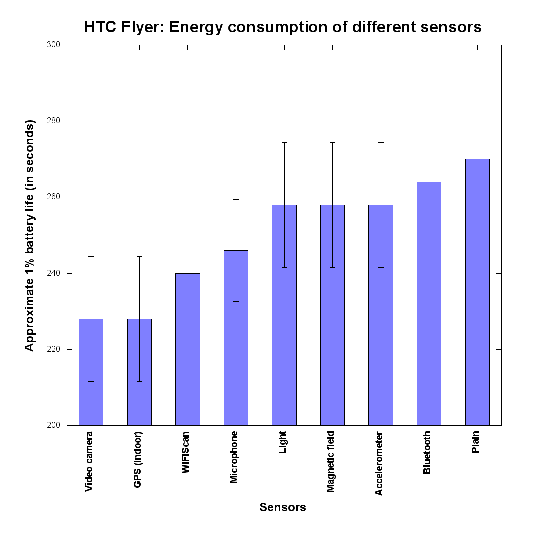
\includegraphics[width=0.49\textwidth, scale=0.6]{plots/htc_flyer}
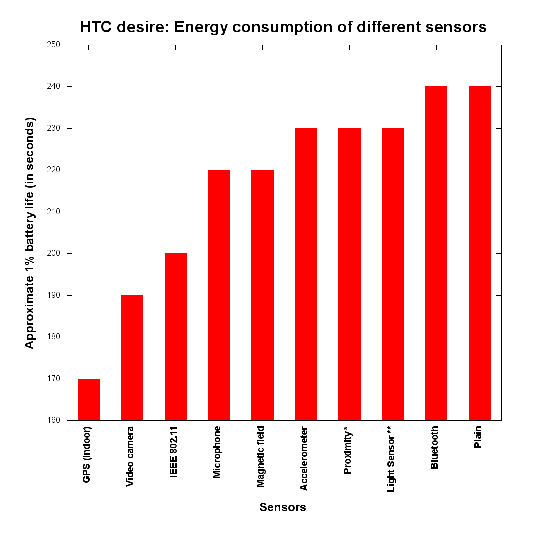
\includegraphics[width=0.49\textwidth, scale=0.6]{plots/htc_desire}
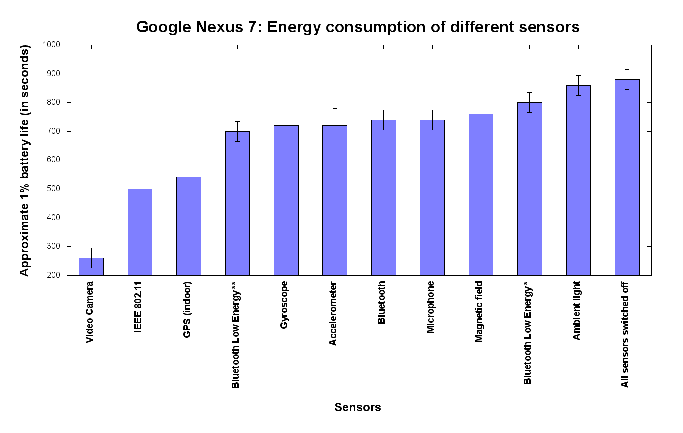
\includegraphics[width=\textwidth, scale=0.9]{plots/google_nexus_7}
\caption{\label{p:all_results} The complete results of energy measurements for all devices. The energy efficiency of different sensors is as expected and overlaps with the results of other research. }
\end{figure}

Bluetooth Low Energy\ (LE) may have higher energy demands than Classic Bluetooth. The \plotref{bluetooth_le_api} compares their energy efficiency depending on the situation. In there is no device found, it takes longer for Bluetooth LE scanning to deplete the battery life by 1\% than for Classic Bluetooth scanning i.e. Bluetooth LE is more energy-efficient. However, if there is any device on the network, Bluetooth LE scanning depletes battery faster than Classic Bluetooth. The reason behind this phenomenon was analyzed in the previous section (the high output of Bluetooth LE API when any device is found) \ref{p:all_results}.
	
\plot{bluetooth_le_api}
				
The energy efficiency order of the sensors differs among the devices. The \plotref{shared} contrasts the energy efficiency results for the shared sensors between the devices.For each of its diagrams, the order of the sensors on x axis is the same. The diagram on the left\ (Google Nexus 7) is characterized by monotonically increasing energy efficiency of the sensors, whereas the other two diagrams are not. For example, Bluetooth is the most energy efficient sensor HTC Desire and HTC Flyer, but is average for Google Nexus 7.

\plot{shared}
		
\subsubsection{Localization}

\hspace{10pt} Different sensors may be used for localization purposes. The \plotref{all_locs} studies the energy efficiency of those sensors. For the comparison, the energy efficiency levels described in the previous section were used. For each of the devices, Bluetooth has the highest energy efficiency level i.e. it is the most energy-efficient. Also, microphone is always more energy efficient than traditional localization sensors\ (GPS and IEEE 802.11). On the other hand, the camera has worse energy performance than GPS and IEEE 802.11 on the two devices. Finally, the energy efficiency of GPS and IEEE 802.11 are similar, though the latter is more energy-efficient for two out of three devices.  	

\plot{all_locs}

Physical sensors are more energy efficient than traditional localization sensors. The energy efficiency of accelerometer is compared with GPS and IEEE 802.11 scanning on the \plotref{acc_vs_loc}. The accelerometer is more energy efficient, but the difference is not always substantial. For HTC Flyer and HTC Desire, the difference between the energy efficiency of accelerometer and traditional localization sensors is less than one energy efficiency level. It is worth reminding here that Accelerometer Sensor Application applies continuous sampling (i.e. sample as often as possible without sleeping intervals).
	
\plot{acc_vs_loc}		

\subsubsection{Conclusions}
\hspace{10pt} The complete set of energy measurements' results are intuitive and overlap with other research, which uses different measurement methods \cite{constandache:localization} \cite{wang:eemss} \cite{chon:smartdc}. This gives validation to the energy measurement method used in this dissertation. For Google Nexus 7, the results confirm the energy-efficiency problems with Bluetooth Low Energy API, which were noticed during the implementation phase. Finally, the energy measurement results vary among different devices. This justifies why the universal power model cannot be used. It also validates the necessity of online energy measurements. 

The analysis of the localization sensors' efficiency explains how localization technologies evolve. Bluetooth, the most energy efficient sensor, is already widely adopted in the industry. iBeacon \cite{apple:ibeacon}, provided by Apple Inc.,  leverages Bluetooth LE for the indoor positioning system. Also, promising energy-efficiency results of microphone attracted research community. SurroundSenses \cite{azizyan:surroundsense} utilizes microphone for localization through ambient sound fingerprinting. Lastly, camera is the most expensive sensor, and thus, computer vision is not yet widely used for localization.

Accelerometer is more energy efficient than traditional localization sensors. Opposite to what previous research\cite{benabdesslem:senseless} stated, the difference in energy consumption is not substantial. The nature of accelerometer usage has been changed. Currently, the values of physical sensors may be pulled more often\ e.g., three accelerometer values are delivered per second on Google Nexus 7. Higher frequency of raw data may have better accuracy, but also results in faster battery depletion.  Because of that, the smarter strategies for sampling needs to be designed. For example, accelerometer may sample for short period of time and if unsure what happens, it could sample longer. As accelerometer has lower energy demands than traditional localization sensors, it could be leveraged for "cheaper" replacement fo those "expensive" sensors. However, its sampling needs to be conducted in energy-efficient manner. 

The energy measurement method does not provide the details on the nature of energy consumption. It is unknown which exact operations consume the most energy during sensing. For example, significant part of energy may be consumed by CPU which needs to be active while sensing accelerometer \cite{priyantha:littlerock}. As those characteristics are not recognized, it cannot be reason how energy efficient the applications with combined sensors\ (IEEE 802.11 scanning and accelerometer) will be. Also, it is unfamiliar how energy efficiency of physical sensors will change depending on their parameters\ (size of sleeping and sampling windows).
						
\subsection{Locy}
-two different scenarios of user movement 
-compared against baseline implementation
	-naive GPS
	-found in the directory..
-compared on three different devices
-each single case sampled three times !

-first scenario: a user sitting in one place whole time
	-outdoor in front of the John Honey building
-the results are in \plotref{locy_eval_inplace}
-Locy performs better for each mobile phone
-why:
	movement detection algorithm is triggered and GPS is switched off all the time
\plot{locy_eval_inplace}

-second scenario: walk for half a time and stand in one place for half a time 
	-outdoor along jack cole building + stopped just in front of john honey building
-the results are in \plotref{locy_eval_other}
-Locy performs better (but not so good like inPlace) or equally good
-why:
	-movement detection algorithm is triggered and switches off GPS after half of the time
	-but through the first phase GPS and accelerometer is being sampled while other application only GPS	
\plot{locy_eval_other}

\subsection{Conclusions}
The energy measurement method delivered the complete set of accurate energy efficiency results, and thus, the method was validated. The results were gathered across three different mobile phones and include all sensors. It is believed that it is the first study of this type. 

Physical sensors could be leveraged for localization purposes. The energy efficiency results gave a basis for how an energy-efficient library could be designed. The energy measurement method provided useful information and identified the challenges for Locy. The energy efficiency of combined sensors and different energy efficiency of physical sensors depending on their parameters needed to be checked. 

Those challenges were met by Locy. The energy-efficient sensing library was evaluated against naive GPS  implementation in two real life scenarios. While a user is staying in one place, Locy is more energy-efficient on three different devices. While a user is walking for half of the time and staying in one place for the rest, Locy outperforms naive GPS implementation. However, the difference is not as significant as in the first scenario.
\section{Conclusions}
\label{s:conc}


Sensor Energy measurement's method:
	-design novel way of investigating energy efficiency
	-checked it in practice, identify its problems
	-the method is validated as the results are compared with other research
	-cons:
		-the method is instable for older batteries 
			-and thus can only be used in limited environment: no online measurement
	
	
Sensor Energy measurement's results:
	-complete set of results across three different phones including all sensors
		-it is believed that the first one like this
	-different energy characteristics across different devices
		->reason for online measurement, invalidate power models
	-the evolution of sensors for localization services
	-cons:
		-no different parameters for phones are checked:
			-no duty cycling checked, no different periods/sleeping intervals checked
	-those results are used to design the energy-efficient algorithms for the library:
		-sensor substitution as cheaper sensor may be leveraged to replace heavy-duty sensors
		-results also raise questions: "combined sensors" -> how they are going to perform?
	
The energy-efficient library:






Future work as well


\bibliographystyle{abbrvDOI}
\bibliography{dissertation}

\appendix
\section{The complete set of experiment samples}
\subsection{Google Nexus 7}	

\begin{table}
    \begin{tabular}{| l | c | c | c |}
    \hline
    Plain                  & 902 & 902 & 841 \\ \hline
    Ambient Light          & 841 & 902 & 841\\ \hline
    Bluetooth Low Energy*  & 782 & 842 & 781 \\ \hline
    Magnetic field:        & 782 & 782 & 721\\ \hline
    Microphone             & 721 & 781 & 782 \\ \hline
    Bluetooth classic      & 781 & 721 & 722 \\ \hline
    Accelerometer:         & 781 & 721 & 661 \\ \hline
    Gyroscope              & 721 & 722 & 721 \\ \hline
    Bluetooth Low Energy** & 722 & 721 & 661 \\ \hline
    \end{tabular}
\end{table}

\subsection{HTC Flyer}	

\begin{table}
    \begin{tabular}{| l | c | c | c | c | c | c | c | c | }
    \hline
    Plain          & \cellcolor{red!25}30  & 270  & 270   & 270   & 271       & 270 & ~      & ~   \\ \hline
    Bluetooth      & 181\^ & 270  & \cellcolor{red!25}30   & \cellcolor{red!25}60   & 270       & 271 & 270      & 241 \\ \hline
    Accelerometer  & 240  & 270  & 180\^ & 271   & 240       & 270 & ~      & ~  \\ \hline
    Magnetic field & 270  & 180\^ & 240   & \cellcolor{red!25}30   & 300^^   & 240 & 270      & 270 \\ \hline
    Light          & 240  & 240  & 271   & 270   & 270       & ~ & ~        & ~   \\ \hline
    Microphone     & 240  & 240  & 240   & 300^^ & 270       & 240 & ~     & ~   \\ \hline
    WiFiScan       & 240  & 241  & 236   & 248 & 240 & ~  & ~   \\ \hline
    GPS            & 241  & 240  & 210 & 240 & \cellcolor{red!25}30 & 210  \\ \hline
    Camera         & 121\^ & 240  & 180^^ & 210   & 241       & 240 & 210      & ~  \\ \hline
    \end{tabular}
\end{table}



\subsection{HTC Desire}	

\begin{table}
    \begin{tabular}{| l | c | c | c | c | c | c | c | c | c | c | c |}
    \hline
    Plain          & 250  & 253  & 251  & 201  & 250  & ~          & ~     & ~   & ~    & ~    & ~   \\\hline
    Bluetooth      & 251  & 251  & 200  & 250  & 250  & ~         & ~     & ~   & ~    & ~    & ~  \\\hline
    Light Sensor** & 251  & 251  & 251  & 200  & 451\^ & 451\^        & 200   & ~ & ~    & ~    & ~  \\ \hline
    Proximity*     & 251  & 501\^ & 451\^ & 200  & 501\^ & 463\^        & 251** & 251 & 403\^ & 401\^ & 200 \\ \hline
    Accelerometer  & 251  & 451\^ & 200  & 401\^ & 200  & 250          & 250   & ~ & ~    & ~    & ~  \\ \hline
    Magnetic Field & 201  & 250  & 201  & 400\^ & 200  & 253          & ~   & ~   & ~    & ~    & ~   \\ \hline
    Microphone     & 400\^ & 200  & 200  & 250  & 200  & 450\^        & 250   & ~ & ~    & ~    & ~   \\ \hline
    WifiScan       & 150  & 300\^ & 251  & 201  & 250  & 151   & ~ & ~    & ~    & ~   \\ \hline
    Camera         & 150  & 200  & 201  & 200  & 200  & ~          & ~     & ~   & ~    & ~    & ~   \\ \hline
    GPS            & 200  & 201  & 150  & 200  & 151  & ~          & ~     & ~   & ~    & ~    & ~   \\ \hline
    Light Sensor*  & 501\^ & 451\^ & 501\^ & 451\^ & 502\^ & ~          & ~     & ~   & ~    & ~    & ~  \\ \hline
    \end{tabular}
\end{table}
\section{Media codecs for sensor measurement applications}
\subsection{Camera application}	
	-Google Nexus 7, HTC desire, HTC flyer:\\
					-Codec H263\\
					-Resolution	176\&144\\
					-Frame rate		~10(HTC flyer),	~12(HTC desire),	~15(Google Nexus 7)\\
					
					
					
\subsection{Microphone application}		
		Google Nexus 7:\\
			-Codec: AMR narrow band(samr)\\
			-channels: 		mono\\
			-sample rate:	8000 Hz\\
			-bits per sample 	32\\
		HTC desire, HTC flyer:\\
			-Codec: AMR narrow band(samr)\\
			-channels:		1\\
			-sample rate:	8000 Hz\\
			-bits per sample:	16\\
			-Bitrate:		128 kb/s	\\
\section{Ethics form}
\label{s:ethicsform}

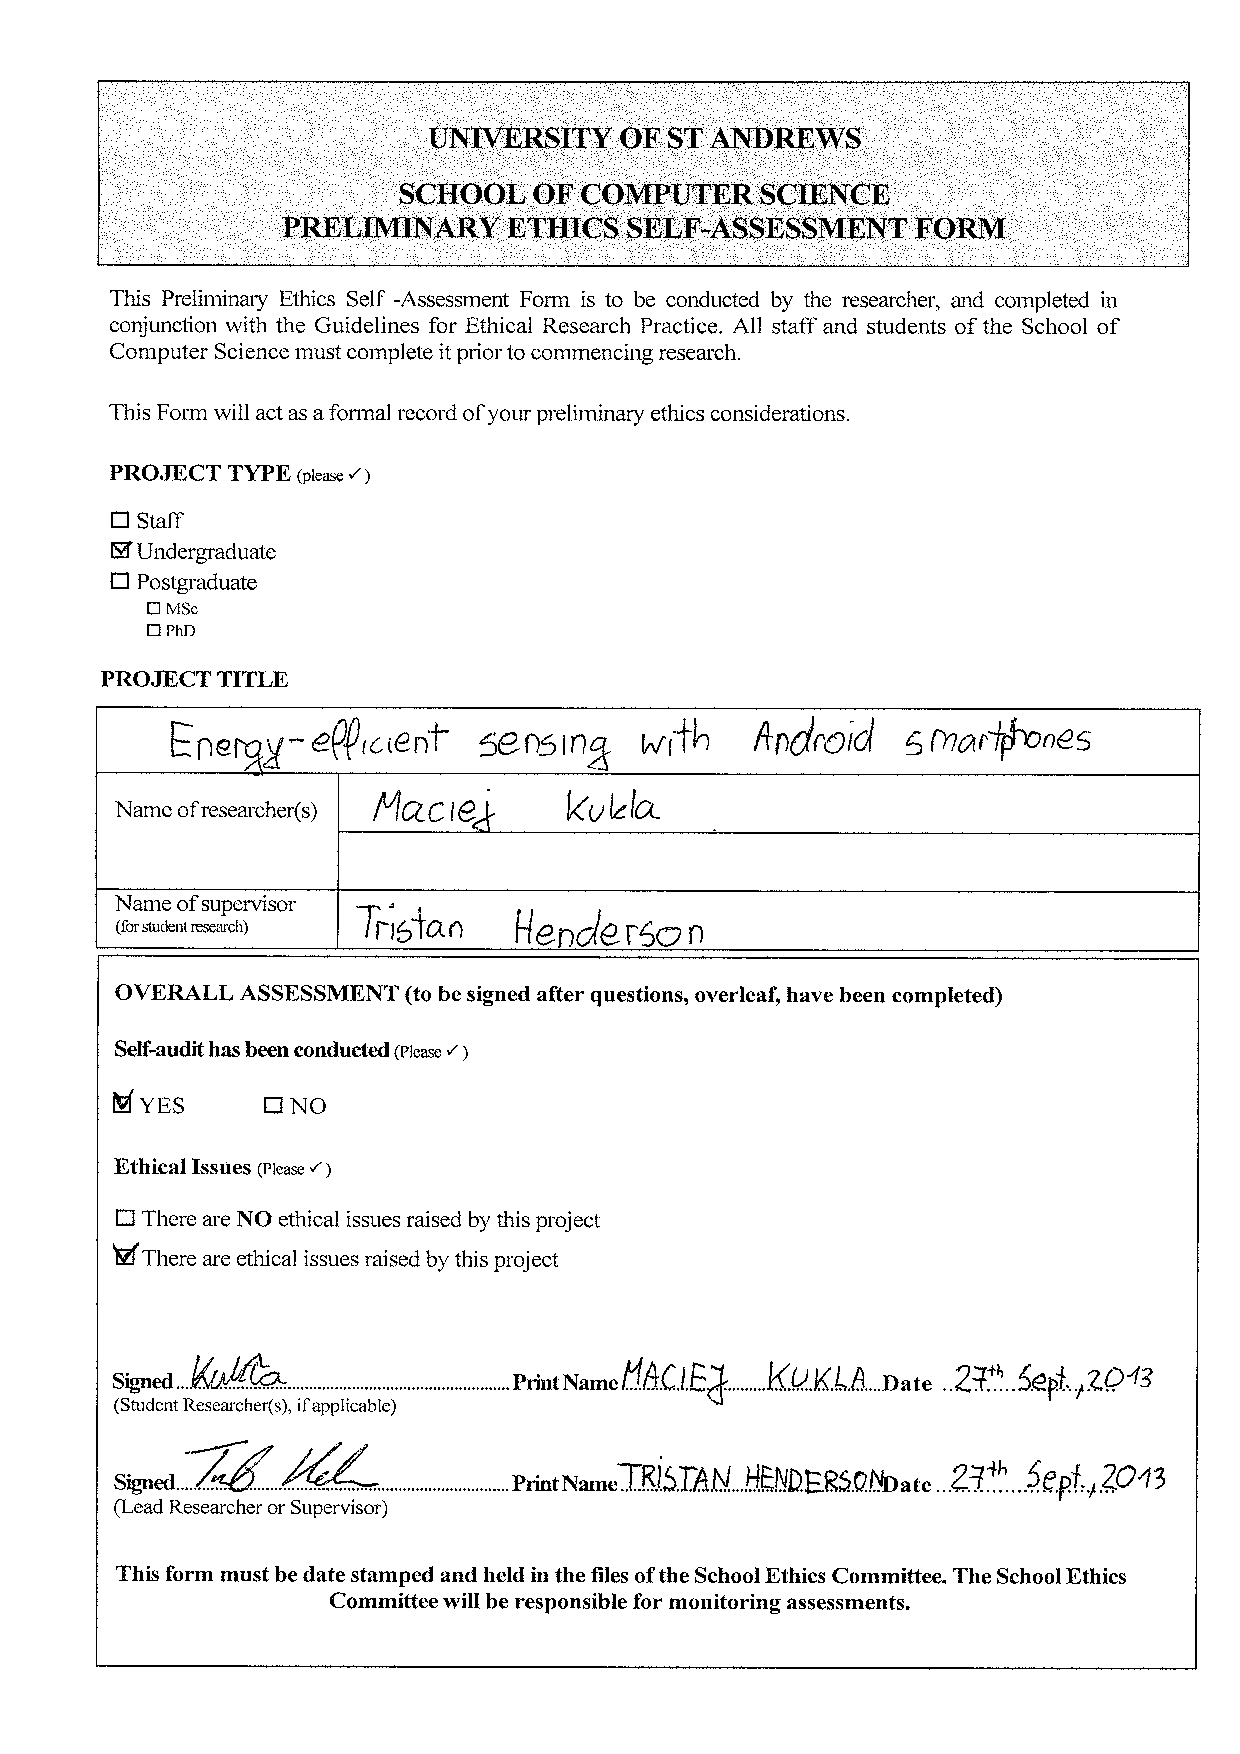
\includepdf[pages={1}]{others/Preliminary_Ethics_Form.pdf}
\includepdf[pages={2}]{others/Preliminary_Ethics_Form.pdf}
\includepdf[pages={3}]{others/Preliminary_Ethics_Form.pdf}
\includepdf[pages={4}]{others/Preliminary_Ethics_Form.pdf}
\end{document}
